\documentclass[10pt, aspectratio=169]{beamer}

% --- PAQUETES ---
\usepackage[utf8]{inputenc}
\usepackage[spanish]{babel}
\usepackage{amsmath}
\usepackage{amsfonts}
\usepackage{xcolor}
\usepackage{tikz}

% --- CONFIGURACIÓN DE DISEÑO PROFESIONAL (LIENZO TRANSPARENTE) ---
\usetheme{default}
\setbeamercolor{background canvas}{bg=}
\setbeamertemplate{navigation symbols}{}
\setbeamertemplate{headline}{}
\setbeamertemplate{footline}{}

% Colores institucionales
\definecolor{unemiAzul}{RGB}{20,40,90}
\definecolor{unemiNaranja}{RGB}{255,102,0}

% Tipografía
\setbeamerfont{frametitle}{size=\Large, series=\bfseries}
\setbeamercolor{frametitle}{fg=unemiAzul}

% --- FONDO DE LA PRESENTACIÓN ---
\setbeamertemplate{background}{
	\begin{tikzpicture}[remember picture, overlay]
		\node[inner sep=0pt] at (current page.center) {
			
\includegraphics[width=\paperwidth, height=\paperheight]{portadaUNEMI2}
		};
	\end{tikzpicture}
}

\begin{document}
	
	% --- PORTADA ---
	{
		\setbeamertemplate{background}{
\includegraphics[width=\paperwidth, height=\paperheight]{portadaUNEMI}}
		\begin{frame}[plain]
			\begin{tikzpicture}[remember picture, overlay]
				\node[fill=unemiAzul, fill opacity=0.8, text opacity=1, rounded corners, inner sep=20pt] at (current page.center) {
					\begin{minipage}{0.7\textwidth}
						\centering
						{\Huge \textbf{\textcolor{white}{Resolución Ejercicio 2}}} \\
						\vspace{0.4cm}
						{\Large \textcolor{white}{Algebra Lineal}} \\
						\vspace{1cm}
						{\small \textcolor{white}{Estudiante:}} \\
						\textbf{\textcolor{unemiNaranja}{Angel Fernando Calero Maldonado}} \\
						\vspace{0.3cm}
						{\small \textcolor{white}{Universidad Estatal de Milagro}}
					\end{minipage}
				};
			\end{tikzpicture}
		\end{frame}
	}
	
	
	% --- DIAPOSITIVA 1 ---
	\begin{frame}{método de Gauss-Jordan matriz inversa}
		
		\vspace{0.35cm}
		
		\makebox[0pt][l]{%
			\hspace*{-1.15cm}
			
			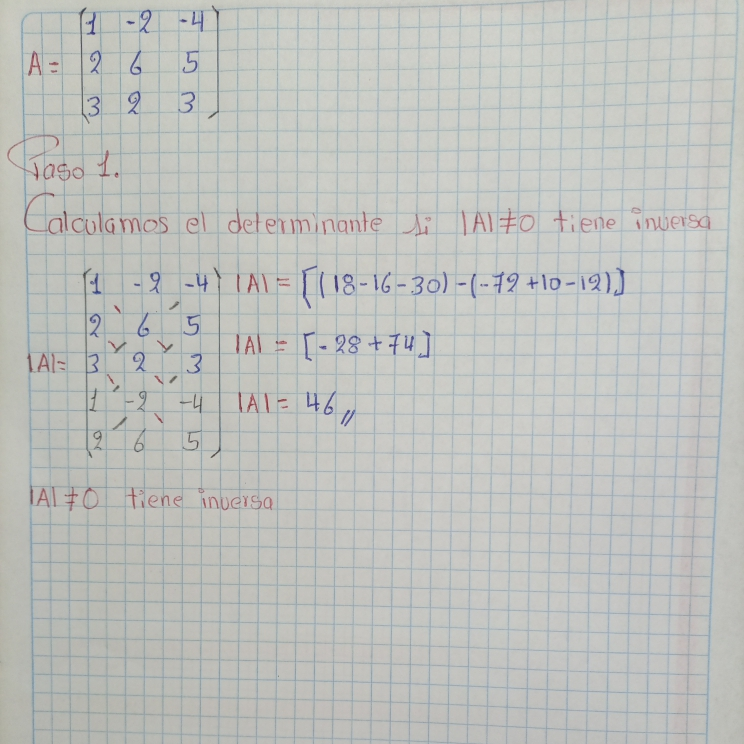
\includegraphics[
			width=\paperwidth,
			height=0.76\paperheight
			]{fotos/foto1.jpeg}
			
		}
		
	\end{frame}
	
	% --- DIAPOSITIVA 2 ---
	\begin{frame}{Matriz Ampliada}
		
		\vspace{0.35cm}
		
		\makebox[0pt][l]{%
			\hspace*{-1.15cm}
			
			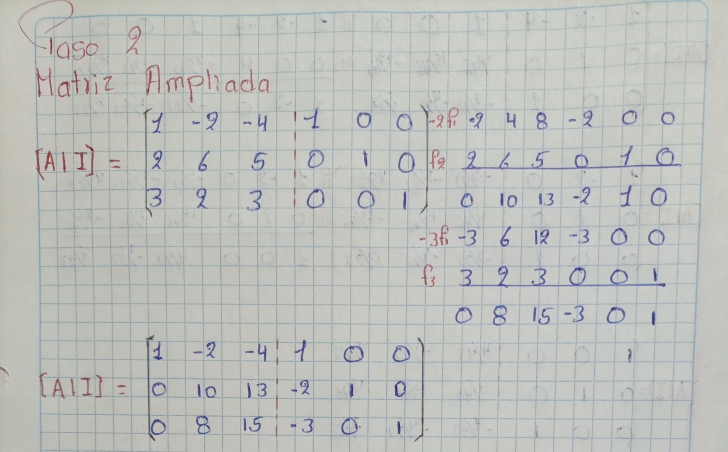
\includegraphics[
			width=\paperwidth,
			height=0.76\paperheight
			]{fotos/foto2.jpeg}
			
		}
		
	\end{frame}
	% --- DIAPOSITIVA 3 ---
	\begin{frame}{Continuación...}
		
		\vspace{0.35cm}
		
		\makebox[0pt][l]{%
			\hspace*{-1.15cm}
			
			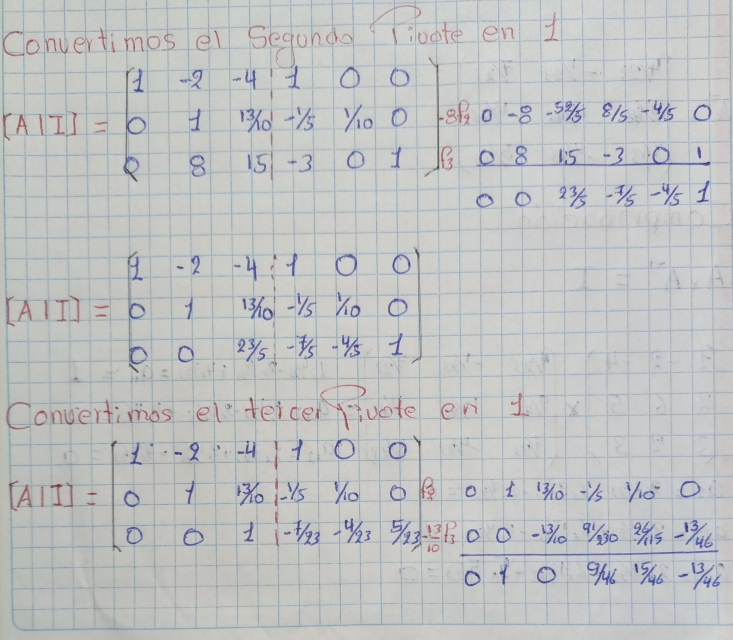
\includegraphics[
			width=\paperwidth,
			height=0.76\paperheight
			]{fotos/foto3.jpeg}
			
		}
		
	\end{frame}
	% --- DIAPOSITIVA 4 ---
	\begin{frame}{Continuación...}
		
		\vspace{0.35cm}
		
		\makebox[0pt][l]{%
			\hspace*{-1.15cm}
			
			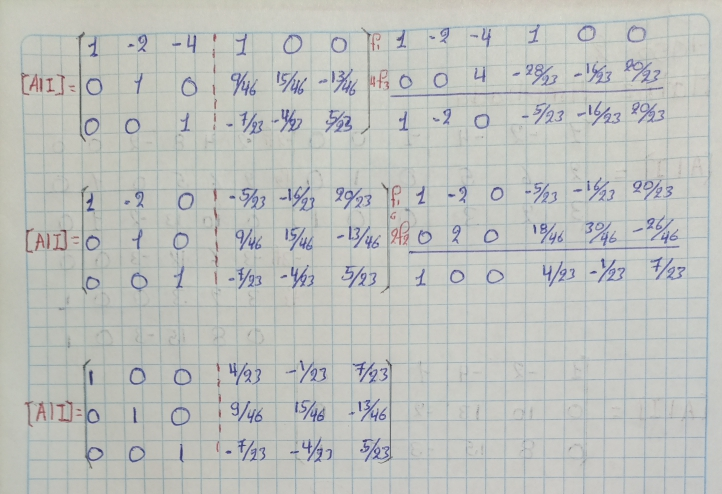
\includegraphics[
			width=\paperwidth,
			height=0.76\paperheight
			]{fotos/foto4.jpeg}
			
		}
		
	\end{frame}
	% --- DIAPOSITIVA 5 ---
	\begin{frame}{Continuación...}
		
		\vspace{0.35cm}
		
		\makebox[0pt][l]{%
			\hspace*{-1.15cm}
			
			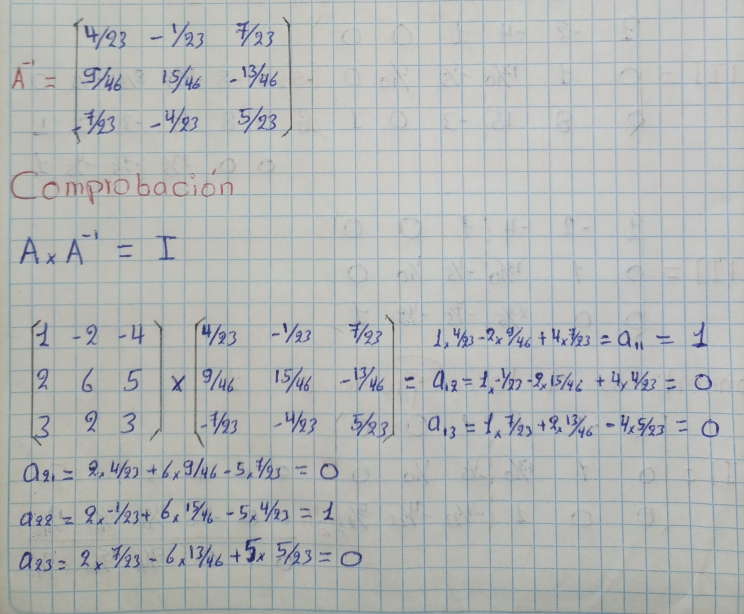
\includegraphics[
			width=\paperwidth,
			height=0.76\paperheight
			]{fotos/foto5.jpeg}
			
		}
		
	\end{frame}
	% --- DIAPOSITIVA 6 ---
	\begin{frame}{Continuación...}
		
		\vspace{0.35cm}
		
		\makebox[0pt][l]{%
			\hspace*{-1.15cm}
			
			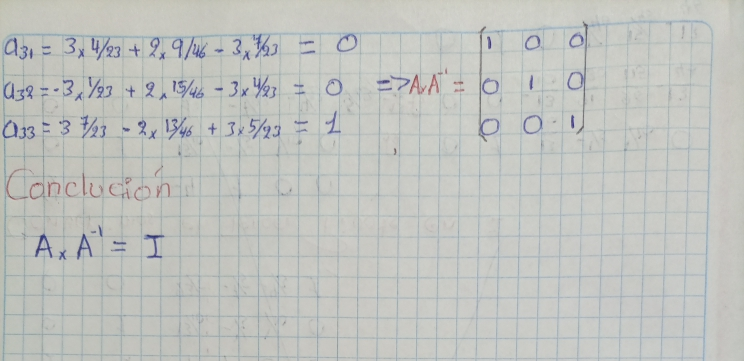
\includegraphics[
			width=\paperwidth,
			height=0.76\paperheight
			]{fotos/foto6.jpeg}
			
		}
		
	\end{frame}
	
	% --- DIAPOSITIVA 7 ---
\begin{frame}{Comprobación}
	
	\vspace{0.35cm}
	
	\makebox[0pt][l]{%
		\hspace*{-1.15cm}
		
		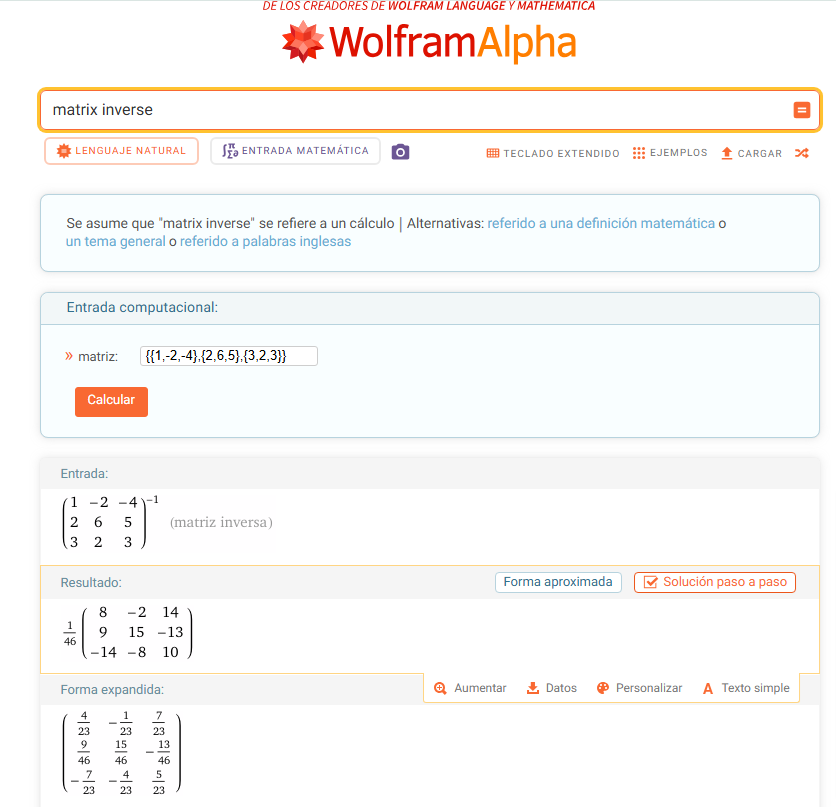
\includegraphics[
		width=\paperwidth,
		height=0.76\paperheight
		]{fotos/comprobar.png}
		
	}
	
\end{frame}
	
	
	% --- DIAPOSITIVA FINAL ---
	{
		\setbeamertemplate{background}{
\includegraphics[width=\paperwidth, height=\paperheight]{portadaUNEMI}}
		\begin{frame}[plain]
			\begin{tikzpicture}[remember picture, overlay]
				\node[fill=unemiAzul, fill opacity=0.8, text opacity=1, rounded corners, inner sep=20pt] at (current page.center) {
					\begin{minipage}{0.9\textwidth}
						\centering
						{\Huge \textbf{\textcolor{white}{Gracias}}} \\
					\end{minipage}
				};
			\end{tikzpicture}
		\end{frame}
	}
	
	
\end{document}